\chapter{Метод взвешанных невязок} \label{chapt3}
\section{Введение}
Цель данной главы --- борьба с одним из артефактов восстановления, так называемым эффектом огрубления пучка или Beam Hardening. 
Одна из причин возникночения таких артефактов --- несоответствие излучения реального источника монохроматическому описанию, используемому в моделях для процедуры восстановления.
Другими словами, физическая модель формирования измерений, используемая при восстановлении, плохо описывает физический процесс измерений.
Для преодоления этого эффекта используют монохроматор --- оптический фильтр, вырезающий определенную линию из спектра.
Однако, проходя через монохроматор, зондирующее излучение сильно уменьшает интенсивность, что влечет за собой увеличение необходимого времени измерения.
Из плюсов использования монохроматора можно отметить более простую фокусировку рентгеновского пучка.
Само по себе использование монохроматора --- сложная инженерная задача \cite{chukalina2014xray}. 
Качественный монохроматор, который не пропускал бы полихроматическую моду к объекту --- сложный и дорогой прибор. 
Так же является трудной задачей юстировка монохроматора.
Поэтому обычно в реальных измерительных схемах стараются обходиться без использования монохроматора.

При этом ПО рекунструкции, поставляемое с томографами, обычно использует монохроматическую модель формирования измерений при восстановлении.
Из-за этого полученный коэффициент поглощения, доставляющий минимум целевой функции, будет содержать артефакты восстановления, например, ложные полости в объекте.
Хотя, как правило, ПО томографов содержит функции исправления подобных артефактов на этапе пред- и постобработки \cite{van2011iterative}, сам физический смысл восстановленной характеристики из линейного коэффициента ослабления веществом рентгеновского излучения на частоте зондирования переходит в некоторый усредненный по спектру коэффициент.
Это может затруднить понимание состава объекта.

Другой возможный способ --- модифицировать механизм реконструкции таким образом, чтобы процедура находилась в соответствии с более точной физиеской моделью.
В данной главе будет предпринята попытка использования априорных знаний об элементном составе объекта для решения задачи восстановления в модели полихроматического зондирования.

\section{Модель томографии при немонохроматическом излучении}

При полихроматическом зондировании спектр излучения источника не сингулярный, а коэффициент ослабления объекта меняется в зависимости от длины волны ($I_0 = I_0(\lambda), f(x, y) = f(x, y, \lambda)$).
Таким образом, при переходе к немонохроматическому случаю, уравнение \eqref{eq:mono_fp} принимает следующий вид:

\begin{equation}
\label{eq:white_fp}
I(l) = \int_0^{+\infty}{\left\{
  I_0(\lambda) \exp{\left(-\int{f(x, y, \lambda) dl} \right) d\lambda} 
  \right\}}.
\end{equation}

Таким образом, оператор проецирования становится нелинейным относительно восстанавливаемой характеристики.
При этом в случае, когда источник все же монохроматический, то есть $I_0(\lambda) = \delta(\lambda - \lambda_0)$ легко видеть, что уравнение (\ref{eq:white_fp}) переходит обратно в (\eqref{eq:mono_fp}).
Спектр используемого в экспериментах источника излучения можно измерить в лабораторных условиях и поэтому считается известным.
Переход к нелинейной задаче не был бы столь существенным, если бы при этом не терялась возможность восстановить зависимость подынтегральной функции от переменной интегрирования. 
Иными словами, без дополнительных знаний о структуре объекта, восстановить искомую функцию $f(x, y, \lambda)$ невозможно.

Предлагается использовать следующую модель формирования функции f. %\cite{?}.
Будем считать, что исследуемый объект состоит из смеси K известных элементов, для которых известны их спектральные функции поглощения $f_k(\lambda)$.
Данные функции измерены для всех распространенных элементов и затабулированы. В частности в данной работе были использованы значения, возвращаемые функциями библиотеки xraylib \cite{xraylib}.
Неизвестными в данной задаче становятся пространственные распределения концентраций $c_k(x, y)$ каждого элемента.
\begin{equation}
 \notag
  f(x, y, \lambda) = \sum_{s=1}^K {c_s(x, y) \cdot f_s(\lambda)},
\end{equation}
т.е. используется аддитавная модель, в которой поглощение на данной длине волны представленно в виде взвешанной суммы поглощиений всех входящих в нее элементов.
Учитывая то, что интеграл внутри экспоненцирования в \eqref{eq:white_fp} --- линейный оператор прямой проекции $H$, получим общее значение ослабления интенсивности входного излучения для смеси $c = (c_1, \dots, c_K)^T $ в пикселе измерения $j$ при линейном размере пикслея $\rho$:
\begin{equation}
  \label{eq:white_fp_final}
  I(c)_j = \int_0^{+\infty} {d\lambda \left\{
    I_0(\lambda) \exp{\left(
      -\sum_{k=1}^K {\rho f_k(\lambda) (H c_k)_j} 
      \right)}
  \right\}}.
\end{equation}

Далее будет предложен итерационный процесс восстановления концентраций, основанный на алгебраическом методе и минимизации $L_2$-нормы относительно неизввестных $c_k$.

\section{Алгебраический метод для немонохроматического случая}
Решение задачи минимизации квадратичной невязки для многомерной задачи будем осуществлять градиентным методом.
Это позволит обеспечить контроль над процедурой оптимизации, а так же обеспечить робастность алгоритма восстановления относительно ошибок измерений.
Цель данного раздела --- вывести формулу для расчета поправки концентраций $c_k$ на каждом шаге итерации метода восстановления.
Индекс $i$, как и ранее, индексирует пиксели в пространстве искомых изображений-концентраций размера $N \times N$.
Индекс $j$ --- пиксели в пространстве входных изображений --- измерений размера $N \times N_\varphi$, а $k \in 1 \dots K$ --- индексирует различные элементы, составляющие исследуемый объект.
Хотя в численных экспериментах будут рассмотрены, в основном, двухкомпонентные смеси, теоретические выводы будут справедливы и для смеси из произвольного числа $K$ компонентов.
Пусть $h_{ij}$ – элементы матрицы прямой томографической проекции H.
Обозначим так же изображение, составленное из измеренний детектора до нормировки и логарифмирования за $t$.

Для того, чтобы выписать минимизационную процедуру необходимо составить функцию невязки.
По аналогии с выводом итерации алгебраического метода для монохроматичного случая, можно взять квадратичную невязку вида $(I(c) - t)^2$.
Однако эта величина размерная и зависит от суммарной мощности просвечивающего пучка.
Поэтому предлагается минимизировать невязку нормированных интенсивностей на величину $ S = \int_0^{+\infty}{I(\lambda)d\lambda}$.
Итак финальная функция для оптимизации имеет вид:
\begin{equation}
\label{eq:white_cost_function}
Q(c) = \left(\frac{I(c) - t}{S}\right)^2,
\end{equation} 
где за возведение в квадрат подразумевается обычная эвклидова норма разницы векторов размера $N \times M_\varphi$.

Для того, чтобы выстроить итерационный процесс вычисления концентраций, необходимо подсчитать градиент весовой функции по концентрациям каждого из элементов. 
Сделаем это покомпонентно:
\begin{equation}
  \notag
  \frac {\partial Q_j} {\partial c_{ki}} = 
  2 \frac {(I(c) - t)_j} {S} 
  \frac {\partial } {\partial c_{ki}}
  \left( \frac {I(c)_j} {S} \right).
\end{equation}

Рассчитаем возникшую частную производную:
\begin{equation}
  \notag
  \begin{split}
  \frac 1 S
  \frac {\partial I(c)_j} {\partial c_{ki}} &= 
  \frac 1 S
  \int_0^{+\infty} {d\lambda \left\{
    I_0(\lambda) 
    \frac \partial {\partial c_{ki}}
    \exp{\left(
      -\sum_{s=1}^K {\rho f_s(\lambda) (H c_s)_j} 
      \right)}
    \right\}} = \\
  &= 
  \int_0^{+\infty} {d\lambda \left\{
    -\rho f_k(\lambda) 
    \frac {I_0(\lambda)} {S}
    \exp{\left(
      -\sum_{s=1}^K {\rho f_s(\lambda) (H c_s)_j} 
         \right)}
    \frac {\partial (H c_k)_j} {\partial c_{ki}}
    \right\}} = \\
  &= 
  \frac {\mu_{kj}} {S} \frac {\partial (H c_k)_j} {\partial c_{ki}},
  \end{split}
\end{equation}

где введено обозначение $\mu_k$ для весовых коэффициентов, имеющих размерность синограммы и зависящих от элемента и прямой проекции:

\begin{equation}
  \label{eq:weights}
  \mu_{k} = \int_0^{+\infty} {d\lambda \left\{
    -\rho f_k(\lambda) 
    I_0(\lambda)
    \exp{\left(
      -\sum_{s=1}^K {\rho f_s(\lambda) (H c_s)} 
         \right)}
    \right\}}
\end{equation}

Эти коэффициенты должны учитывать спектральное взаимодействие различных элементов с источником, взвешивая невязку для каждого элемента, благодаря чему на каждой итерации вклад в разные концентрации будет разный.

Заметим, что производная $\frac {\partial (H c_k)_j} {\partial c_{ki}}$ соответствует обратной проекции в алгебраической процедуре восстановления. 
Таким образом, шаг итерации будет иметь вид
\begin{equation} \label{eq:part3_whitegrad}
  \nabla_k \ Q = 2H^\intercal R_k \text{, где } R_{kj} = \frac {(I(c) - t)_j} {S^2} \mu_{kj},
\end{equation}

где за $R_k$ обозначена взвешенная невязка для элемента $k$. 
Таким образом, мы вычислили компоненты градиента по каждому из составляющих исходный объект элементу.
Как видно из формулы \ref{eq:part3_whitegrad}, компоненты градиентов по различным элементам могут вычисляться отдельно.
Тем не менее, не стоит забывать, что все элементы связаны через взвешенные невязки $R_k$ , в которых содержится зависимость от всего вектора $c$.
Итак, наконец, шаг итерации алгоритма выглядит следующим образом:
\begin{equation}
  \label{white_iteration}
  c_k^\xi = c_k^{\xi - 1} - \gamma_k (\xi - 1) H^\intercal R_k(c_k^{\xi - 1}).
\end{equation}

\section{Мультикомпонентная регуляризация}
Несмотря на полученный шаг градиентного спуска, решение минимизационной задачи для функции \eqref{eq:white_cost_function} невозможно простым градиентным спуском.
Это можно проиллюстрировать на следующем примере.
Рассмотрим упрощенную задачу на изображении размера 1x1 пиксель, одна измеренная проекция. 
Пусть этот объект зондируется монохроматическим излучением, и состоит из смеси двух компонентов, с поглощающими способностями и концентрациями $\alpha_1, c_1$ и $\alpha_2, c_2$, соответственно.
Тогда восстановление сведется к решению уравнения вида $ \alpha_1 c_1 + \alpha_2 c_2 = p$
Этому уравнению удовлетворяет любое решение, лежащее в координатах $c_1, c_2$ на отрезке, соединяющем точки $(0, \frac{p}{\alpha_2}$ и $(\frac{p}{\alpha_1}, 0)$.
Несмотря на это, градиентная оптимизация, начатая из точки $(0, 0)$ приведет в точку $(p\frac{\alpha_1^2}{\alpha_1^2 + \alpha_2^2}, p\frac{\alpha_2^2}{\alpha_1^2 + \alpha_2^2})$.
Независимо от того, какой реально элемент присутствовал в пикселе, ответом будет некоторый усредненный состав, с долями, пропорциональными полгощающей способности элемента (см. рис. \ref{fig:c1_c2_plot}).

\begin{figure}
  \centering
  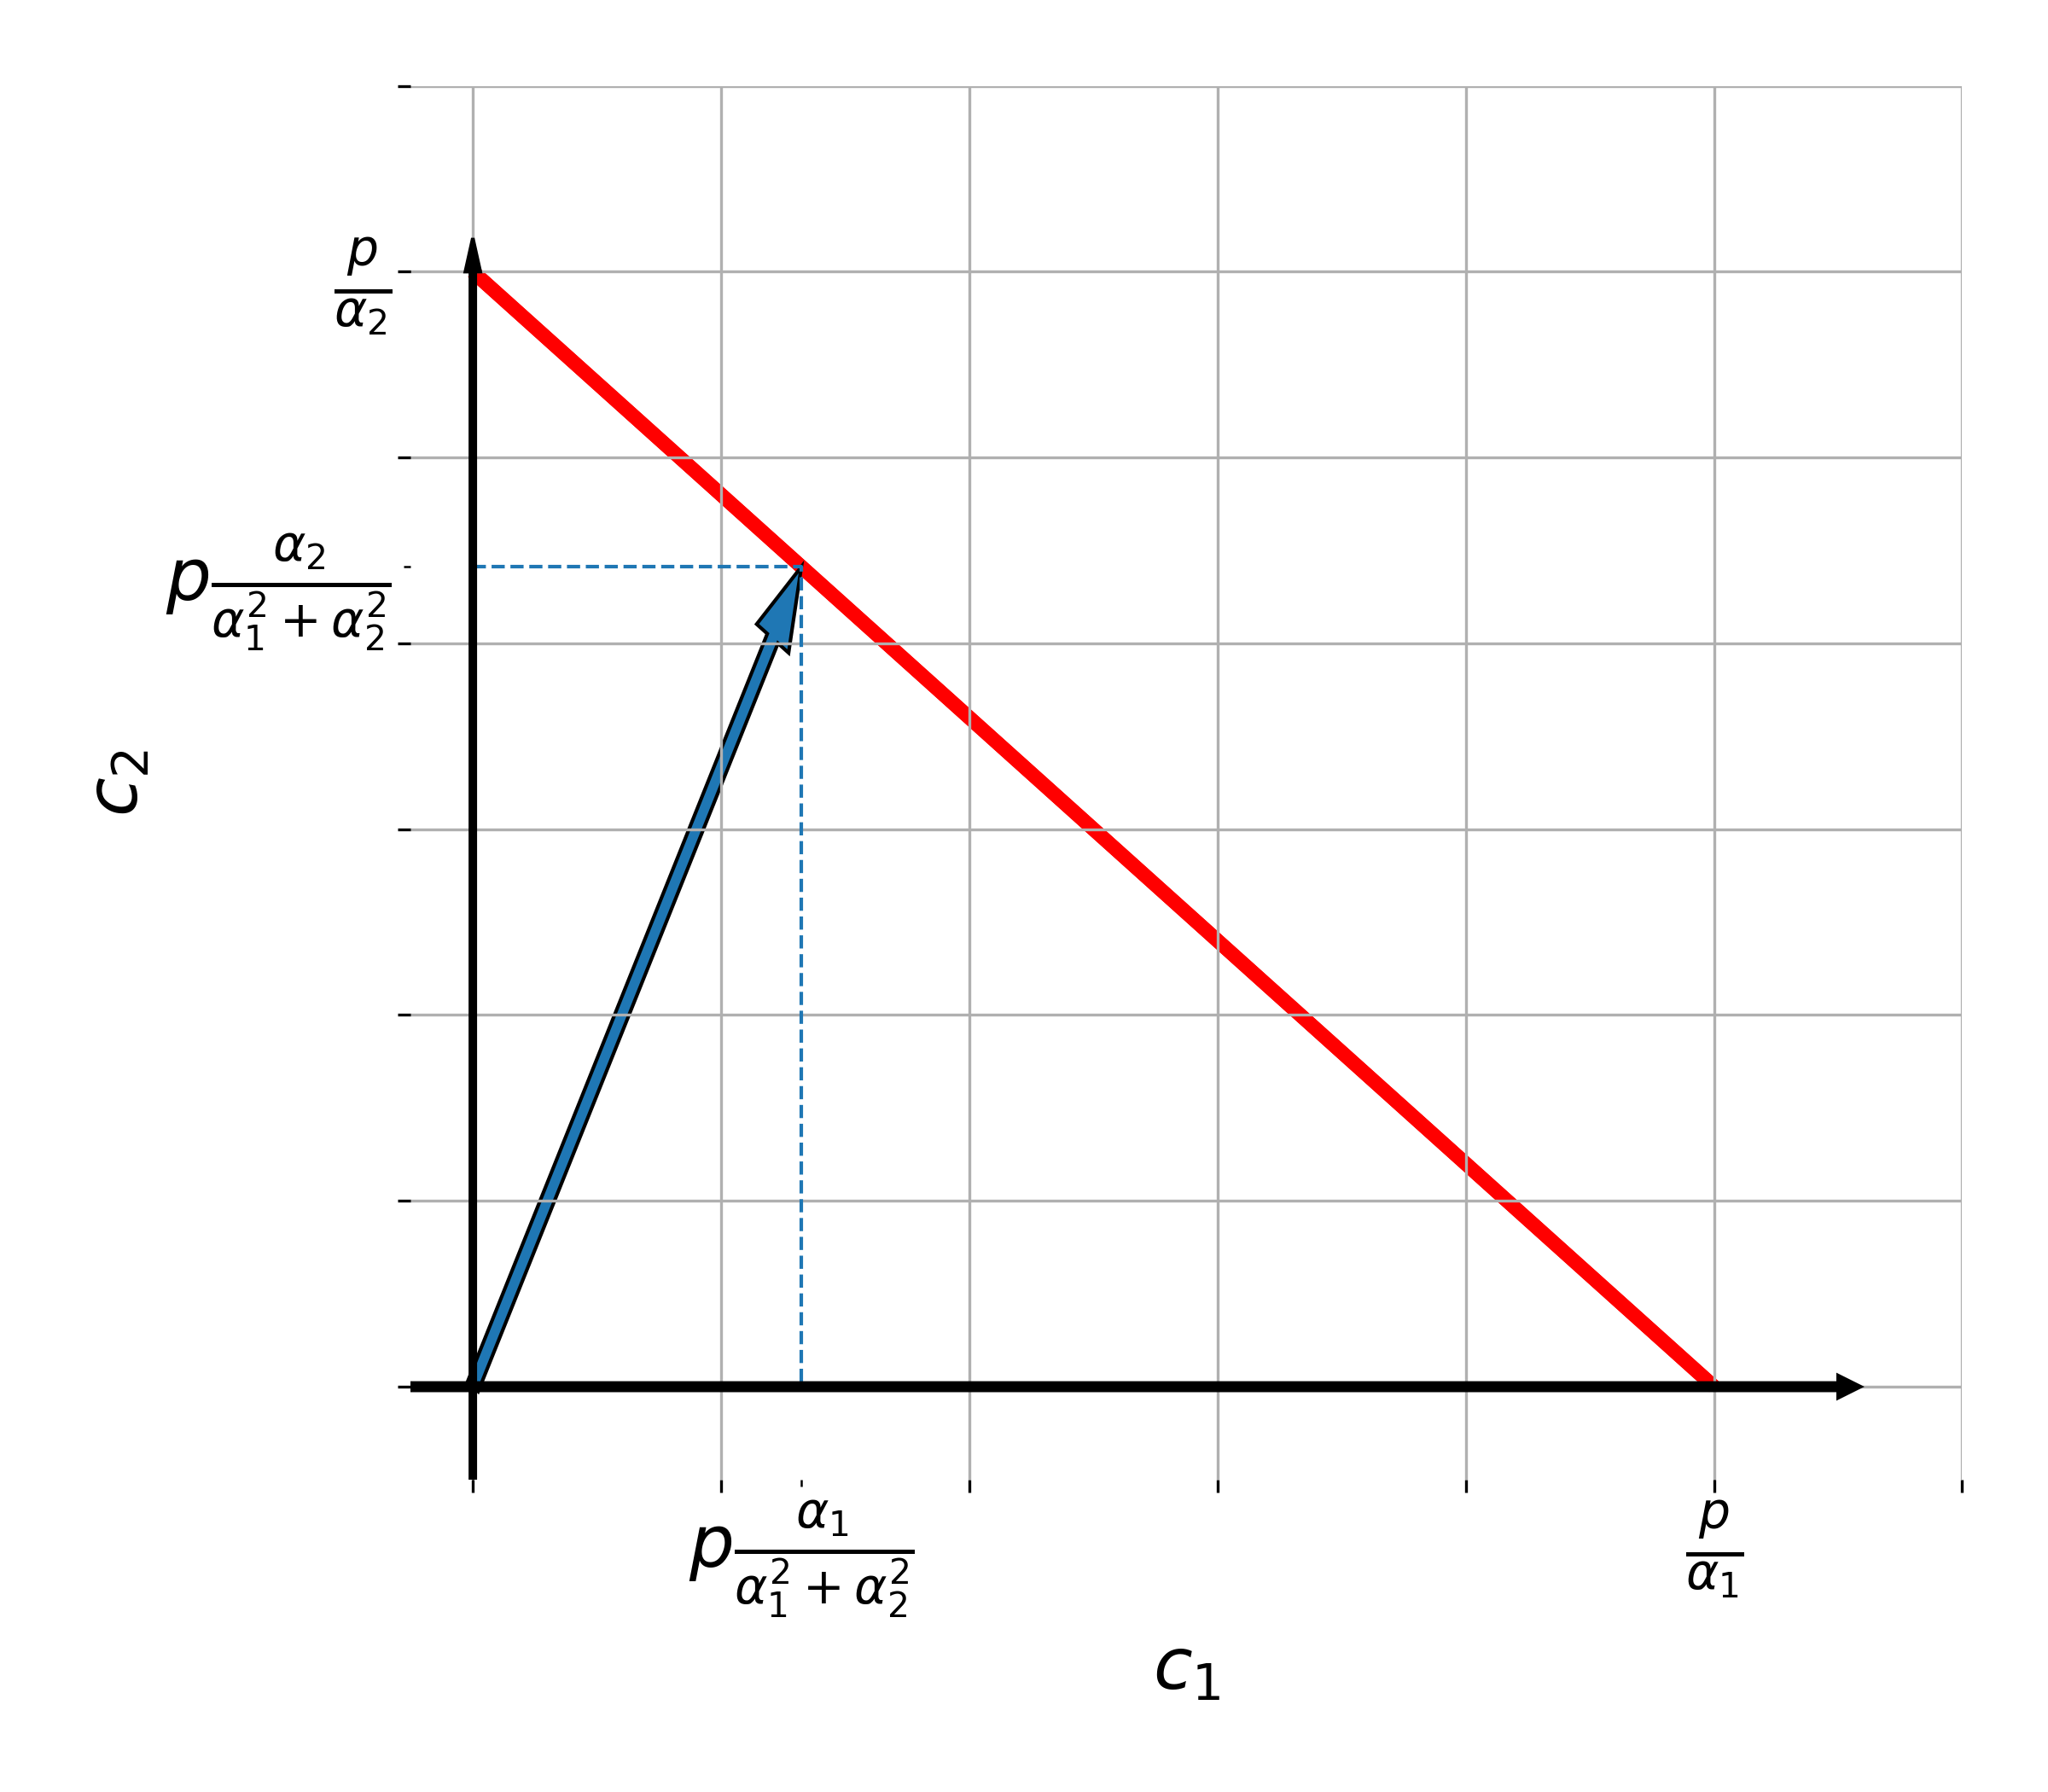
\includegraphics[width=0.8\textwidth]{part3_img/c1_c2_plot}
  \caption{Градиентная процедура минимизации не может найти истинное соотношение концентраций.}
  \label{fig:c1_c2_plot}
\end{figure}

Этот пример иллюстрирует невозможность градиентной процедурой пространствено ``разделить'' концентрации разных элементов в задаче.
Однако ситуацию можно исправить, если ввести априорное предположение о том, что в одном пикселе сканируемой площади может находиться только один элемент из смеси.
Данное условие можно сформулировать в виде уравения $c_1(x,y) * c_2(x,y) = 0 \forall x,y$ для двух элементов.
Введя операцию поэлементного умножения векторв $(\cdot \odot \cdot)$, и записав $\frac{K(K-1)}{2}$ ограничений для всех пар, получится $c_{k} \odot c_{s} = 0$, если $k \neq s$.

Данные ограничения-неравенства предлагается добавить в виде аддитивных квадратичных штрафов в функционал оптимизации.
Так же учтем, что концентрации принимают значения в интервале от 0 до 1 в виде ограничений-неравенств.
Финальный вид оптимизационной задачи МВН \eqref{eq:wrm_opt}:

\begin{equation}
\label{eq:wrm_opt}
  \begin{cases}
    \begin{array}{lc}
    Q(c) + \beta\sum_{k_1 != k_2}\Norm{c_{k_1} \odot c_{k_2}} \to \min \limits_c & w.r.t \\
    c_k \geq 0 & \\
    c_k \leq 1
    \end{array}
  \end{cases}.
\end{equation}

Для решения оптимизационной задачи с ограничениями-неравенствами \eqref{eq:wrm_opt} применяется метод барьерных функций \eqref{eq:quadprog_barrier}.
Для того, чтобы добиться наиболее разного поведения для переменных $c_1$ и $c_2$ применялись дополнительно следующие меры.
Во-первых, начальные значения для концентраций инициализируются семлированием пикселей из случайных обрезанных нормальных величин (truncated normal distribution).
Этот подход часто используется, например, при обучении нейронных сетей градиентными методами обратного распространения ошибки и помогает оптимизации избежать выхода на ``плато''

Другой подход для того чтобы повысить неоднородность восстановления заключался в том, чтобы с одного шага градиента обновлять не все изображение $c_k$, а лишь некоторую произвольную подобласть изображения.
Подобласть выбиралась двумя способами: мозаичным и гауссовым.
В первом изображение делилось на некоторое фиксированное число квадратных подобластей, и активная подобласть просто случайным образом выбиралась.
Это приводит к появлению мозайчатых артефактов на ``стыках'' областей.
Второй --- к плавному прибавлению градиента, ослабленного гауссовым окном со случайным центром.
Этот подход позволяет получить более мягко сглаженную картину, однако в результате все равно появляются характерные артефакты, в виде максимумов интенсивности в произвольных местах.
Более того, такие методы сильно замедляют сходимость метода, т.к. из всего вычисленного градиента используется только малая часть.

\section{Численный эксперимент}
Описанный алгоритм и регуляризации были имплементированы в рамках комплекса программ whitomo \cite{whitomo}.
Поведение алгоритма и результаты восстановления были рассмотрены на примере как синтетических фантомов, измерения которых были результатми компьютерной симуляции, так и реальных экспериментальных данных.
Все эксперименты были проведены для смеси из двух компонент.

В качестве фантомов рассматривались различные простые конфигурации из окружностей и эллипсов.
В рамках разработанного ПО реализована возможность выбора различной конфигурации а так же спектральных функций поглощения элементов, составляющих объект.
Для экспериментов с синтетическими данными использовался модельный спектр и характеристики поглощения, продемонстрированные на рис. \ref{fig:synth_spectrum}.
Спектр имеет пики на энергиях 2.5 и 10 кэВ, которые совпадают с пиками поглощения обоих элементов.

\begin{figure}
\centering
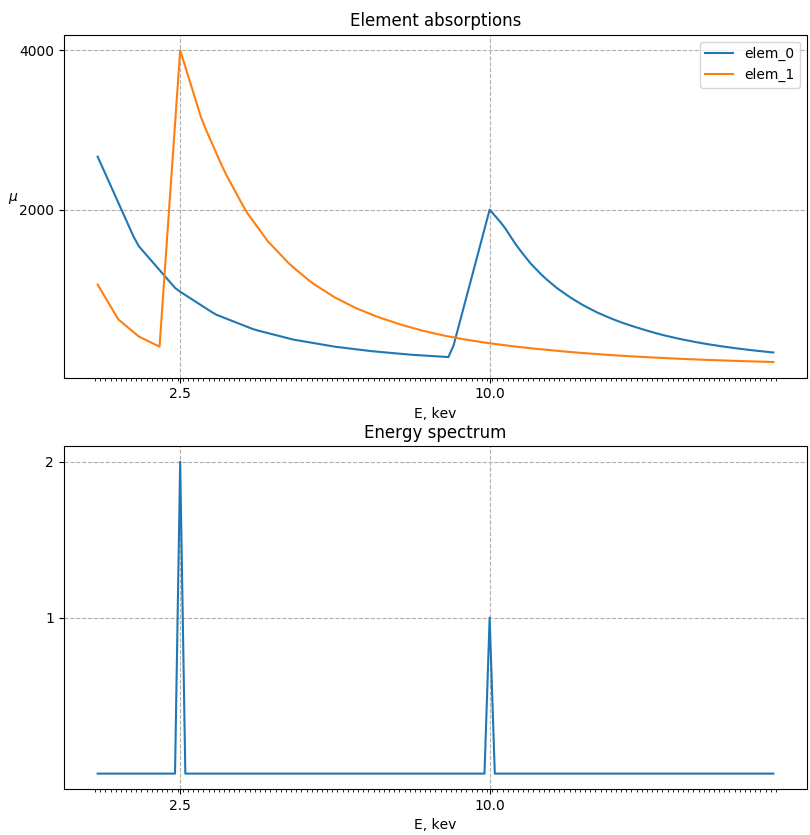
\includegraphics[height=0.5\textheight]{part3_img/synth_spectre}

\caption{Спектр зондирования и массовые коэффициенты ослабления элементов для симуляций измерений фантомов.}
\label{fig:synth_spectrum}
\end{figure}

Форма используемых фантомов и результаты восстановления методом взвешанных невязок приведены на рис. \ref{fig:synth_recon}.
Реконструкция способна пространственно разделить объекты разных элементов, т.е. восстановленные концентрации $c_1, c_2$ отличаются больше чем на константу.
Восстановленные объекты видны на картинах концентраций.
На картине концентрации слабопоглощающего элемента присутствуюты артефакты восстановления: ``тень'' от другого объекта а так же сам пик концентрации не достигает истинного значения 1.0.

\begin{figure}
\centering
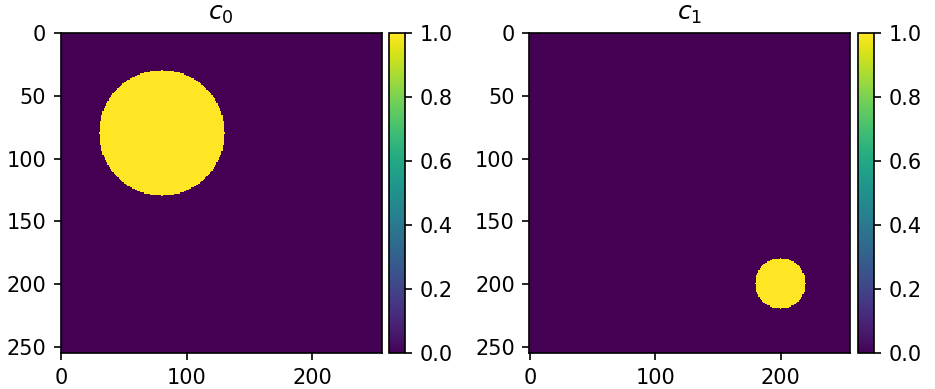
\includegraphics[width=\textwidth]{../Presentation/images/0999}
\\
a)
\\
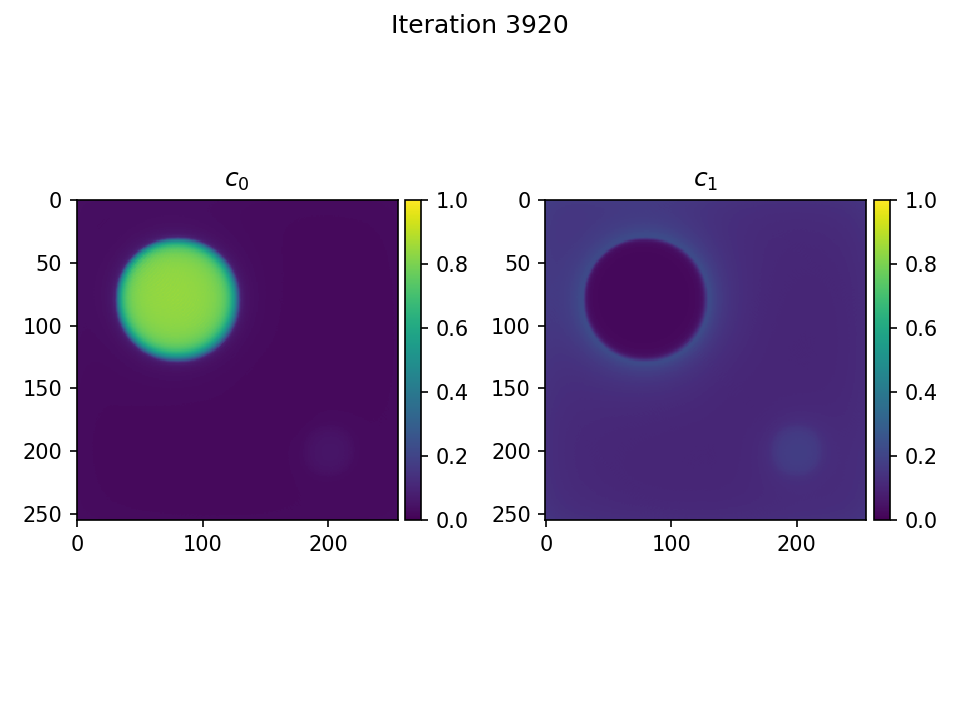
\includegraphics[width=\textwidth]{../Presentation/images/whiterec_res}
\\
б)
\\
\caption{Результаты эксперимента с синтетическими данными: а) фантом. б) восстановление}

\todo{отображение на одной картинке концентраций различных элементов}

\todo{кросс-секции вдоль диагонали}
\label{fig:synth_recon}
\end{figure}

\todo{восстановление зуба}

\todo{выводы по главе}

\todo{нормальное заключение}

\todo{побольше ссылок про полихроматику в литобзор}

\begin{comment}
\section{Численный Эксперимент} \label{sect_3_2}
Одним из результатов данной главы является программная реализация и исследование работы алгоритма восстановления, основанного на взешенных невязках.
Алгоритм был реализован на языке python с использованием библиотеки ASTRA \cite{van2015astra}.
Для восстановления были использованы различные конфигурации модельных данных, так и модельные данные (фантом), состоящий из двух овальных областей, имеющих пересечение и состоящих из элементов номер 22 и 28.
Распределения концентраций элементов представлены на рисунке \ref{fig:white_phantom}




%\begin{figure}
%\begin{subfigure}[h]{0.45\textwidth}
%  \centering
%    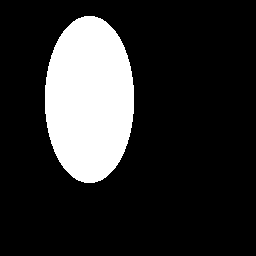
\includegraphics[width=\textwidth]{part3_img/c_22}
%  $c_22$
%\end{subfigure}
%\begin{subfigure}[h]{0.45\textwidth}
%  \centering
%    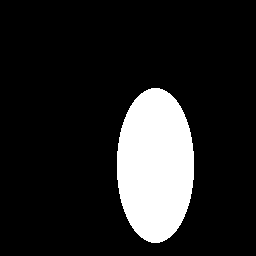
\includegraphics[width=\textwidth]{part3_img/c_28}
%  $c_28$
%\end{subfigure}
%  \caption{Используемые для симуляций концентрации}
%\label{fig:white_phantom}
%\end{figure}

\begin{figure}
  \centering
\begin{tabular}{@{}c@{}c}
    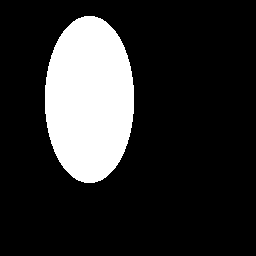
\includegraphics[width=0.45\textwidth]{part3_img/c_22}
  &
    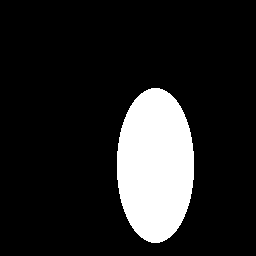
\includegraphics[width=0.45\textwidth]{part3_img/c_28}
  \\
    $c_22$ & $c_28$
\end{tabular}
  \caption{Используемые для симуляций концентрации}
\label{fig:white_phantom}
\end{figure}


На рисунке \ref{fig:source} представлены спектры поглащения элементов и спектр испускания выбранного для симуляций источника.

\begin{figure}
  \centering
  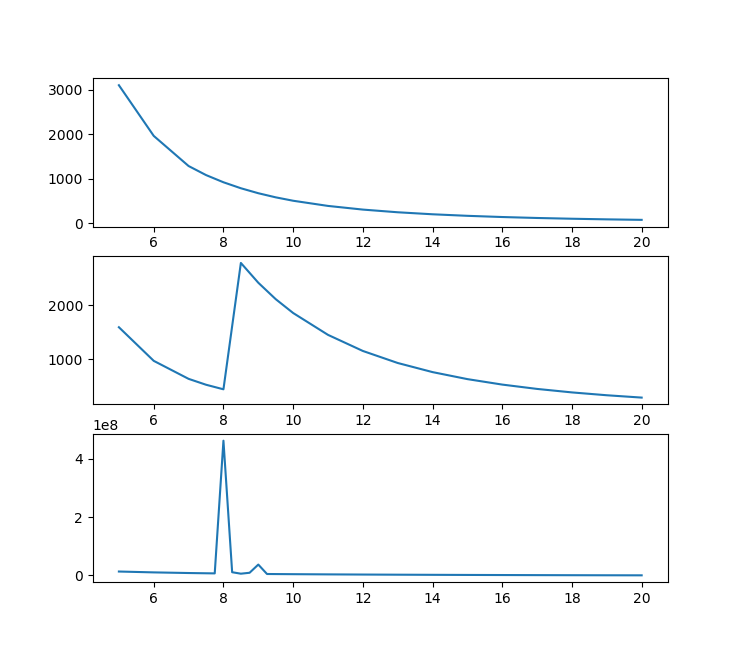
\includegraphics[width=0.95\textwidth]{part3_img/graphs}
  \caption{Сверху вниз: коэффициент поглощения для элементов 22, 28 и спект источника}
  \label{fig:source}
\end{figure}

При проведении первых симуляций оказалось, что восстановление итерационными методами сходится к локальному минмуму мультиспектральной задачи.
Это проявляется в том, что промежуточные концентрации в результате градиентного спуска приходят в вырожденному решению, не содержащему специфики элементов, из которых состоит образец.
Обе концентрации получаются равномерно размазанными по площади, занятой объектом, с характерными артефактами --- лишним увеличением концентрации вдоль выпуклой оболочки \ref{fig:wrart_noreg_25}.
Вырождение состоит в том, что значения концентраций отличаются в константу раз равномерно по всей площади восстанавливаемых концентраций.

\begin{figure}
  \centering
  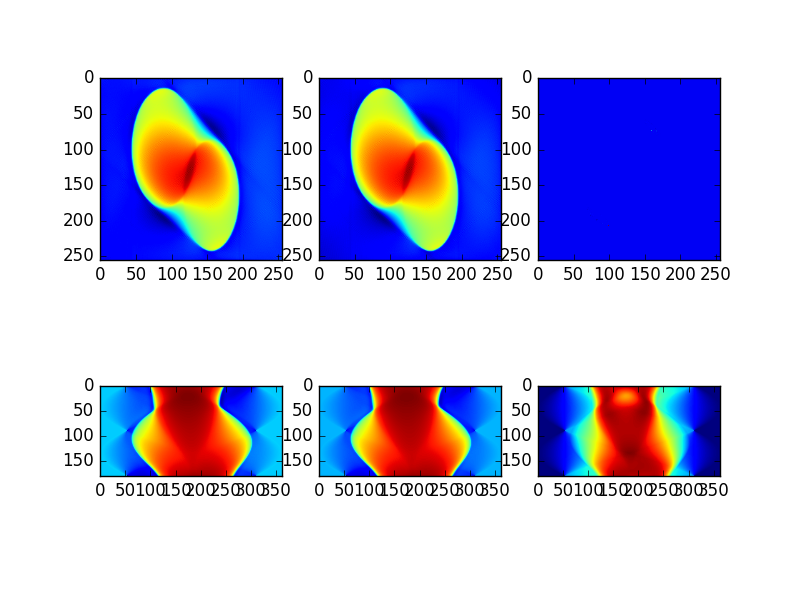
\includegraphics[width=0.95\textwidth]{part3_img/no_reg_iteration_25}
  \caption{Восстановление с помощью МВН, концентрации и их отношение, их синограммы и отношения}
  \label{fig:wrart_noreg_25}
\end{figure}

\todo{вывести соотношение, к которому выраждаются восстановленные картины}

\section{Полихроматическая регуляризация}
\todo{описать подробно регуляризацию модуля произведений}

Вырождение концентраций различных элементов легко проиллюстрировать следующим примером.

\todo{сингулярный спектр, сингулярные кривые поглащения двух элементов. реконструкция - решение уравнения с 2 неизвестными. график в координатах c1, c2, решение лежит на отрезке между осями в положительном квадранте (для некоторого пикселя). вырождение идет к прямой $c_1 = \alpha c_2$. Нужно запретить это - одновременно нельзя обеим концентрациям быть положительными. Иными словами, $c_1 c_2 = 0$}

Логичным ограничением при оптимизации является запретить находиться в одном пикселе восстанавливаемой площади концентраций двух разных элементов.
Чтобы ввести такое ограничение, можно перейти к задаче условной оптимизации, добавив ограничение $c_1 c_2 = 0$ или, в случае $K$ различных элементов $\frac{ K (K - 1) } { 2 }$ ограничений вида $c_{k_1} c_{k_2} = 0, k_1 \neq k_2$.
Так же можно добавить условия на положительность концентраций $c_k \geq 0$.
В результате восстановление томографии в полихроматической моде сведется к оптимизации с ограничениями.
Следуя логике раздела \ref{sect_2_2}, заменяя жесткие ограничения-равенства на мягкие, получаем что регуляризация может быть получена добавлением в целевую функцию штрафов за модуль произведения концентраций. 
Дополнительно добавляется мягкий штраф за отличие значений концентраций от 0 и 1, подобно тому как это сделано в \cite{svets2016}: $||c - 0.5||^2$
\todo{описать подробнее}

Результаты восстановления с использованием такой мультипликативной регуляризации (мягких ограничений-равенств условной оптимизации) представлены на рисунке \ref{fig:wrart_mulreg_150}

\begin{figure}
  \centering
  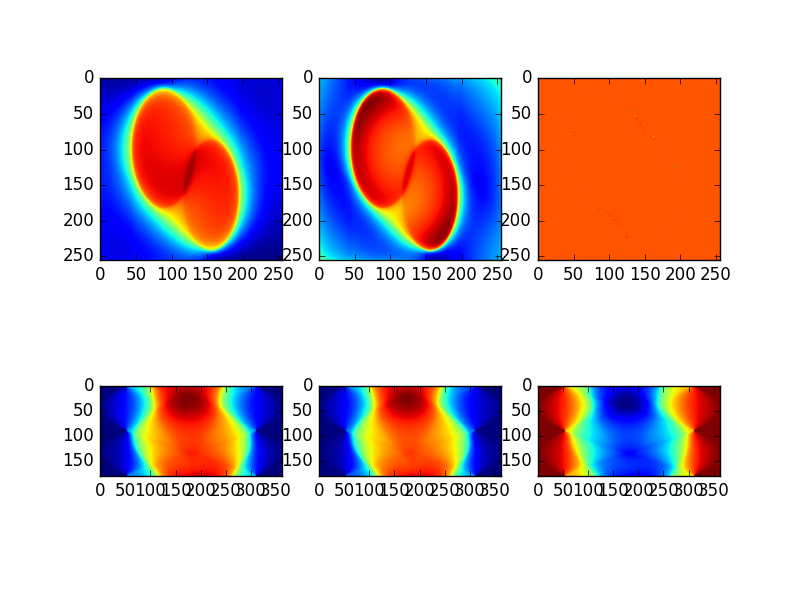
\includegraphics[width=0.95\textwidth]{part3_img/mul_reg_iteration_150}
  \caption{Восстановление с помощью МВН с использованием мультипликативной регуляризации}
  \label{fig:wrart_mulreg_150}
\end{figure}

\todo{описать переход к вырожденному спектру}

\end{comment}

\section{Выводы} \label{sect_3_3}
